\subsection{Experimental Setup}
We organize the evaluation around three questions that correspond to the main control points in the \ours lifecycle:
\begin{enumerate}
    \item \textbf{Offline evolution.} Can historical trajectories be distilled into a cold-start skill library that transfers to unseen tasks?
    \item \textbf{Online evolution.} Can the library accumulate useful experience over a sequential task stream?
    \item \textbf{Recommendation.} Given a skill library, does task-conditioned recommendation outperform exposing the library wholesale?
\end{enumerate}

\paragraph{Benchmarks.}
We evaluate \ours with Harbor on Terminal-Bench 2.0 and SWE-Bench Pro public \citep{harborFramework,merrill2026terminal,deng2025swe}. Terminal-Bench 2.0 contains 89 difficult terminal tasks inspired by real workflows; SWE-Bench Pro public contains 731 long-horizon software-engineering tasks from 11 public repositories. Following the leaderboards, we report avg@5 Accuracy and avg@1 Resolve Rate, respectively, ordering SWE-Bench Pro tasks by repository. Terminal-Bench Pro supplies offline data: we retain 48 public software-engineering and system-administration tasks, excluding 2 environment-unstable tasks \citep{wang2025let}.

\paragraph{Configurations.}
All settings use Codex with \texttt{GPT-5.2} or \texttt{GPT-5.4 mini} \citep{openai2025gpt52,openai2026gpt54MiniNano}. Both benchmarks include a no-skill baseline and an online setting that starts empty and evolves with task-level recommendation. Terminal-Bench 2.0 also includes an offline setting: a library is first built from 48 Terminal-Bench Pro historical tasks, with evolution triggered after every 4 tasks; the frozen library is then transferred to Terminal-Bench 2.0 for recommendation only.

\subsection{Main Results}
Tables~\ref{tab:main-results-tb2} and~\ref{tab:main-results-swebenchpro} report the main performance. On Terminal-Bench 2.0, \ours improves Accuracy in both offline and online settings. Offline evolution gives the clearest signal: a frozen library distilled from 48 Terminal-Bench Pro trajectories transfers to unseen tasks, improving GPT-5.2 by \svgain{+7.9 pp} and GPT-5.4 mini by \svgain{+5.8 pp}. This suggests that trajectory-derived skills can form a useful cold-start library rather than merely capturing source-task artifacts.

Online evolution yields smaller but positive gains. Starting from an empty library, \ours improves Terminal-Bench 2.0 Accuracy by \svgain{+2.7 pp} with GPT-5.2 and \svgain{+1.1 pp} with GPT-5.4 mini. On SWE-Bench Pro, online evolution improves Resolve Rate for both backbones: GPT-5.2 rises from 47.6 to 50.2, a \svgain{+2.6 pp} gain, and GPT-5.4 mini rises from 46.9 to 49.0, a \svgain{+2.1 pp} gain. These gains are heterogeneous across difficulties and repositories, indicating that online skill accumulation is useful but sensitive to the evidence observed early in the task stream.

\begin{table}[t]
    \caption{Main results on Terminal-Bench 2.0. Scores are avg@5 Accuracy; deltas denote absolute percentage-point changes from the corresponding no-skill baseline.}
    \label{tab:main-results-tb2}
    \centering
    \scriptsize
    \setlength{\tabcolsep}{4pt}
    \renewcommand{\arraystretch}{1.5}
    \begin{tabular}{
        >{\raggedright\arraybackslash}m{0.20\linewidth}
        >{\raggedright\arraybackslash}m{0.11\linewidth}
        >{\raggedright\arraybackslash}m{0.085\linewidth}
        >{\raggedright\arraybackslash}m{0.095\linewidth}
        >{\raggedright\arraybackslash}m{0.085\linewidth}
    }
        \toprule
        \multirow{2}{*}{\textbf{Model / Setting}} & \multicolumn{1}{c}{\underline{\textbf{Overall}}} & \multicolumn{1}{c}{\textbf{Easy}} & \multicolumn{1}{c}{\textbf{Medium}} & \multicolumn{1}{c}{\textbf{Hard}} \\
        & \multicolumn{1}{c}{\footnotesize (89)} & \multicolumn{1}{c}{\footnotesize (4)} & \multicolumn{1}{c}{\footnotesize (55)} & \multicolumn{1}{c}{\footnotesize (30)} \\
        \specialrule{\lightrulewidth}{\aboverulesep}{0pt}
        \rowcolor{black!8}
        \multicolumn{5}{c}{Codex} \\
        GPT-5.2 Medium & 51.0 & 75.0 & 54.9 & 40.7 \\
        \quad \online & 53.7\svup{2.7} & 75.0 & 62.9\svup{8.0} & 34.0\svdown{6.7} \\
        \quad \offline & 58.9\svup{7.9} & 90.0\svup{15.0} & 65.1\svup{10.2} & 43.3\svup{2.7} \\
        \arrayrulecolor{black!25}\hdashline\arrayrulecolor{black}
        GPT-5.4 mini Medium & 51.7 & 75.0 & 61.8 & 30.0 \\
        \quad \online & 52.8\svup{1.1} & 75.0 & 63.6\svup{1.8} & 30.0 \\
        \quad \offline & 57.5\svup{5.8} & 65.0\svdown{10.0} & 64.7\svup{2.9} & 43.3\svup{13.3} \\
        % \midrule
        % \rowcolor{black!8}
        % \multicolumn{5}{c}{Claude Code} \\
        % Claude 4.5 & -- & -- & -- & -- \\
        % \quad \online & -- & -- & -- & -- \\
        % \quad \offline & -- & -- & -- & -- \\
        \bottomrule
    \end{tabular}
\end{table}

\begin{table*}[t]
    \caption{Main results on SWE-Bench Pro public. Scores are avg@1 Resolve Rate; deltas denote absolute percentage-point changes in the overall column.}
    \label{tab:main-results-swebenchpro}
    \centering
    \scriptsize
    \setlength{\tabcolsep}{3pt}
    \renewcommand{\arraystretch}{1.7}
    \resizebox{\textwidth}{!}{%
    \begin{tabular}{
        >{\raggedright\arraybackslash}m{1.1in}
        >{\raggedright\arraybackslash}m{0.52in}
        ccccccccccc
    }
        \toprule
        \multirow{2}{*}{\textbf{Model / Setting}} & \multicolumn{1}{c}{\underline{\textbf{Overall}}} & \textbf{ansib.} & \textbf{openl.} & \textbf{quteb.}
        & \textbf{flipt} & \textbf{telep.} & \textbf{vuls} & \textbf{navid.}
        & \textbf{webcl.} & \textbf{eleme.} & \textbf{nodeb.} & \textbf{tutan.} \\
        & \multicolumn{1}{c}{\footnotesize (731)} & \footnotesize (96) & \footnotesize (91) & \footnotesize (79)
        & \footnotesize (85) & \footnotesize (76) & \footnotesize (62) & \footnotesize (57)
        & \footnotesize (65) & \footnotesize (56) & \footnotesize (44) & \footnotesize (20) \\
        \specialrule{\lightrulewidth}{\aboverulesep}{0pt}
        \rowcolor{black!8}
        \multicolumn{13}{c}{Codex} \\
        GPT-5.2 Medium
        & 47.6 & 49.0 & \textbf{64.8} & 62.0 & 32.9 & 34.2 & 54.8 & \textbf{49.1} & \textbf{43.1} & 50.0 & 47.7 & 0.0 \\
        \quad \online
        & 50.2\svup{2.6} & \textbf{56.2} & 63.7 & \textbf{68.4} & 32.9 & \textbf{35.5} & \textbf{56.5} & 45.6 & 38.5 & 50.0 & \textbf{72.7} & 0.0 \\
        \arrayrulecolor{black!25}\hdashline\arrayrulecolor{black}
        GPT-5.4 mini Medium
        & 46.9 & \textbf{52.1} & 55.0 & 64.6 & 31.8 & 35.5 & 50.0 & \textbf{50.9} & 38.5 & 46.4 & 61.4 & 0.0 \\
        \quad \online
        & 49.0\svup{2.1} & 51.0 & \textbf{59.3} & \textbf{68.4} & \textbf{32.9} & \textbf{38.2} & \textbf{56.5} & 49.1 & 38.5 & \textbf{51.8} & 61.4 & 0.0 \\
        % \midrule
        % \rowcolor{black!8}
        % \multicolumn{13}{c}{Claude Code} \\
        % Claude 4.5
        % & -- & -- & -- & -- & -- & -- & -- & -- & -- & -- & -- & -- \\
        % \quad \online
        % & -- & -- & -- & -- & -- & -- & -- & -- & -- & -- & -- & -- \\
        \bottomrule
    \end{tabular}%
    }
\end{table*}


\subsection{Analysis}

\noindent
The main results show that \ours improves frozen agents on both terminal and software-engineering tasks, but the gains are not uniform across settings. We therefore analyze where the gains come from and when skills become harmful. The analysis follows the three control points of the \ours lifecycle: pre-task exposure control, post-task evolution from historical evidence, and cross-task transfer of the evolved procedures.

\Needspace{0.50\textheight}
\subsubsection{Recommendation Controls Negative Transfer}
\begin{wrapfigure}{r}{0.40\columnwidth}
    \vspace{-0.8\baselineskip}
    \centering
    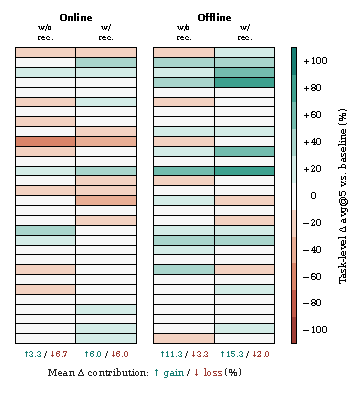
\includegraphics[width=\linewidth]{assets/tb2_hard_ablation.pdf}
    \caption{Recommendation ablation on Terminal-Bench 2.0 Hard subset. Each cell shows task-level avg@5 change over the no-skill baseline; recommendation filters harmful skill exposure and improves the gain/loss balance.}
    \label{fig:tb2-hard-rec-ablation}
\end{wrapfigure}

Figure~\ref{fig:tb2-hard-rec-ablation} studies whether a skill library should be exposed directly or mediated by task-conditioned recommendation. The central observation is that skill exposure is not neutral. When the online library is exposed without recommendation, negative task-level deltas outweigh positive ones: the mean gain/loss contribution is \svgain{$+3.3$}/\svloss{$-6.7$}. With recommendation, the early online library is still not a strong source of improvement, but the net negative effect disappears, yielding \svgain{$+6.0$}/\svloss{$-6.0$}. This suggests that, in the early online regime, recommendation mainly acts as a noise filter: it prevents sparse, under-specified, or weakly related skills from entering the solver context.

The offline setting gives a cleaner view of the same mechanism. The transferred library is already useful without recommendation, but recommendation increases the mean positive contribution from \svgain{$+11.3$} to \svgain{$+15.3$} and reduces the loss from \svloss{$-3.3$} to \svloss{$-2.0$}. Thus, evolution and recommendation play complementary roles. Evolution creates potentially reusable procedural knowledge, while recommendation decides whether that knowledge should be exposed to the current task. This also explains why the average gains in Tables~\ref{tab:main-results-tb2} and~\ref{tab:main-results-swebenchpro} are moderate despite large improvements on some tasks: skills create a heavy-tailed effect, helping substantially when matched well but causing regressions when exposed indiscriminately.

\FloatBarrier
\subsubsection{Offline Evolution Accumulates Transferable Procedures}
\begin{figure}[!b]
    \centering
    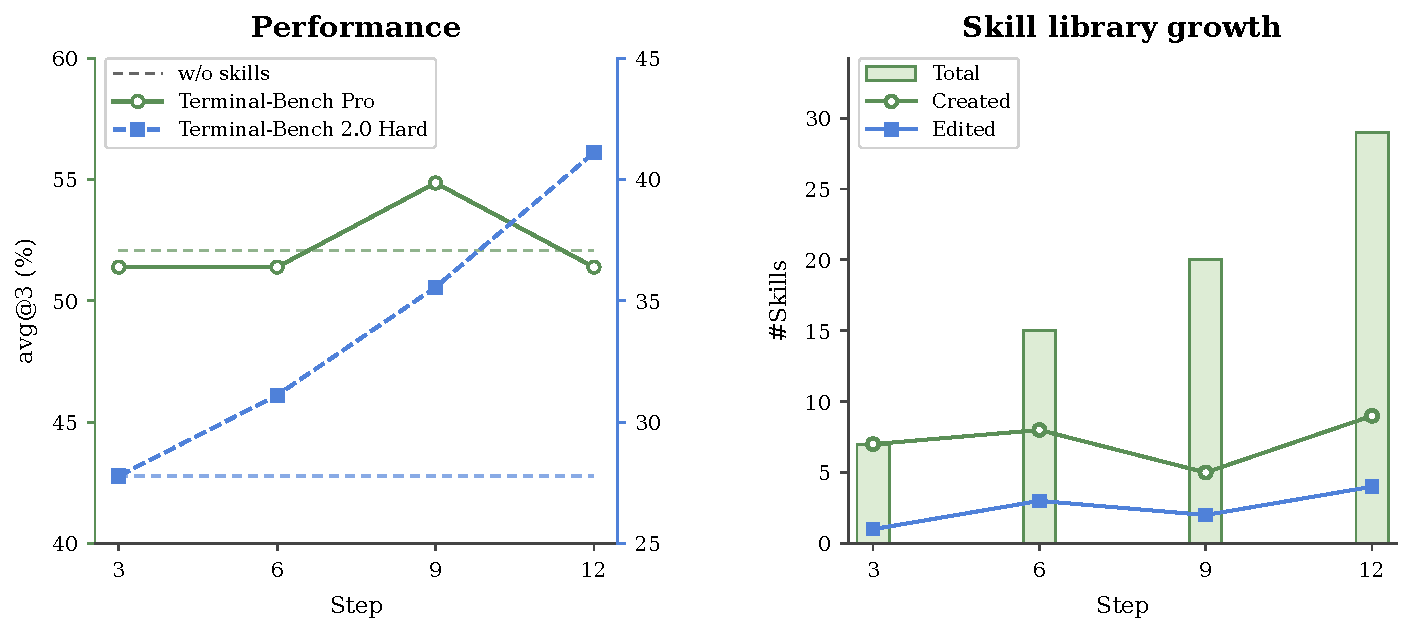
\includegraphics[width=.8\linewidth]{assets/evolve_dynamics.pdf}
    \caption{Evolution dynamics of the offline skill library on Terminal-Bench Pro. Left: checkpointed libraries are evolved on Terminal-Bench Pro and transferred frozen to Terminal-Bench 2.0 Hard subset; curves report avg@3. Right: library growth includes both new skill creation and edits to existing skills.}
    \label{fig:evolve-dynamics}
\end{figure}

Offline evolution does not optimize the source benchmark score directly. Ground-truth and verifier signals are used only after task completion to support attribution: they help determine which parts of the trajectory were successful, reusable, and properly attributable. The evolution stage then consumes the attributed subtask records rather than oracle answers, and benchmark-specific constants or gold outputs are excluded from reusable exploration.

Figure~\ref{fig:evolve-dynamics} reflects this separation. Terminal-Bench Pro performance fluctuates across checkpoints, whereas the frozen libraries transfer increasingly well to unseen Terminal-Bench 2.0 Hard tasks. The non-monotonic source-side curve separates source-task performance from transfer-side library utility: \ours is not simply fitting the source benchmark. The transfer-side improvement suggests that the library accumulates reusable operational procedures that survive task distribution shift. The library-growth panel further shows that evolution is not append-only trajectory storage. New skills are created, but existing skills are also edited, indicating that \ours consolidates repeated evidence into persistent skill artifacts.

\subsubsection{Case Study: What Transfers Across Tasks}
\begin{figure}[t]
    \centering
    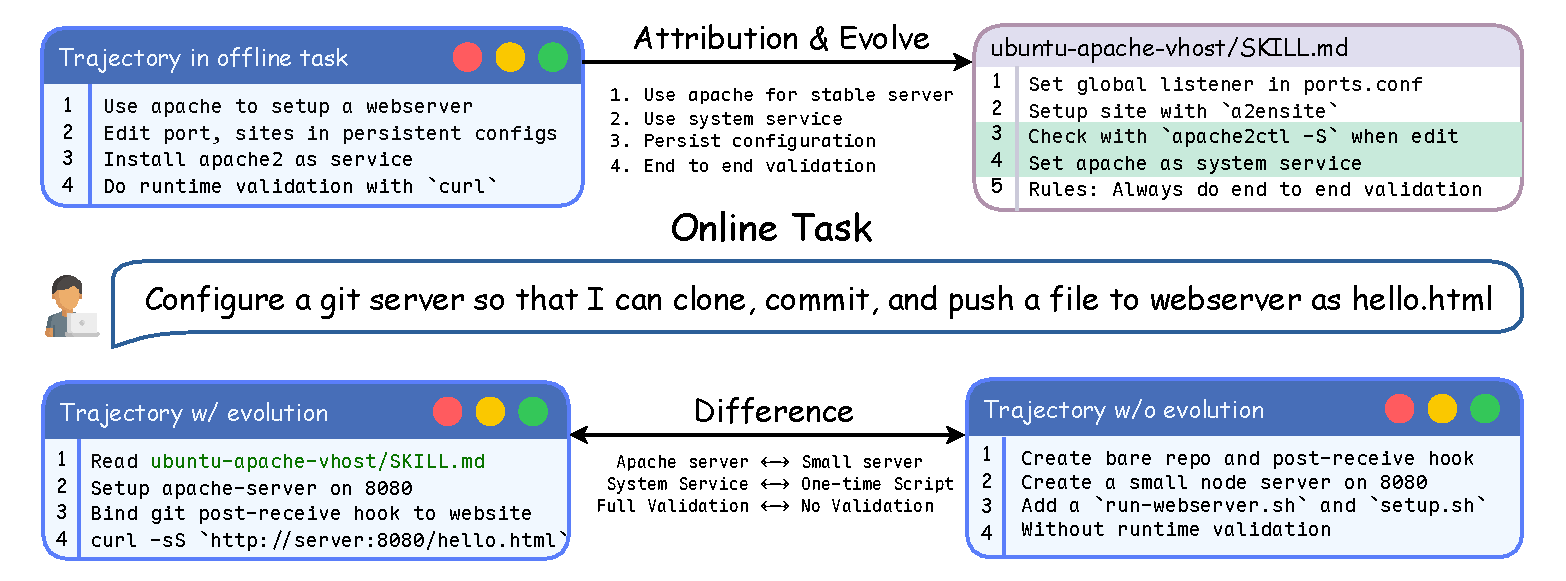
\includegraphics[width=.8\linewidth]{assets/evolve_demo.pdf}
    \caption{Representative offline-transfer case. A skill evolved from an Apache website task transfers persistent-service setup and end-to-end validation to an unseen Git-server deployment task.}
    \label{fig:offline-transfer-case}
\end{figure}

Figure~\ref{fig:offline-transfer-case} provides a representative example of what is transferred by offline evolution; the source offline-evolution trajectories are shown in Appendix~\ref{app:case-apache-logging-rat} and~\ref{app:case-apache-analytics-virtu}. The source trajectories implement Apache-backed websites and contribute reusable knowledge about persistent Apache configuration, service installation, and end-to-end runtime validation. These lessons are distilled into the \texttt{ubuntu-apache-vhost} skill rather than stored as raw trajectories.

On the unseen Git-server task, whose trajectory is shown in Appendix~\ref{app:case-apache-git}, the evolved run does not copy the source solution. Instead, it reuses the operational pattern: deploy the web endpoint with a stable Apache service, connect the Git post-receive hook to the served directory, and validate the full path by requesting the final URL. The baseline run builds a bare repository and a lightweight Node server, but it lacks persistent service setup and final runtime validation. The case illustrates the type of transfer that \ours is designed to preserve: not task-specific constants or answers, but reusable execution invariants that improve reliability on a different task.

\FloatBarrier
